%----------------------------------------------------------------------------
\chapter{Repülési hálózat vizsgálata}\label{test}
%----------------------------------------------------------------------------
Ebben a fejezetben az \href{http://openflights.org/}{openflights.org} oldalon elérhető repülési adatbázis feldolgozását és ezen adatokon futtatott szimulációt mutatom be.

  %----------------------------------------------------------------------------
  \section{Az adatok}
  %----------------------------------------------------------------------------
  Az \href{http://openflights.org/}{openflights} lehetőséget biztosít különféle repülési adatok interaktív keresésére, regisztráció után pedig akár statisztikákat készíthetünk saját utazásainkról. Emellett elérhető a mindenkori aktuális, teljes adatbázisa is, amit többek között hivatalos forrásokból és a felhasználóktól gyűjt.
  Az oldalon elérhető adatbázis világszerte mindenhonnan gyűjt és tárol repülőtéri, repülőtársasági és repülési út adatokat. Több, mint 9000 repülőtér, 19000 társaság és közel 60000 repülési út érhető el. Részletes adatok \aref{tab:table_repterek}.,~\aref{tab:table_repulesitarsasagok}., és a \aref{tab:table_repulesiutvonalak}. táblázatokban.

    %----------------------------------------------------------------------------
    \subsection{Repülőterek}
    %----------------------------------------------------------------------------
    \begin{figure}[!ht]
      \centering
      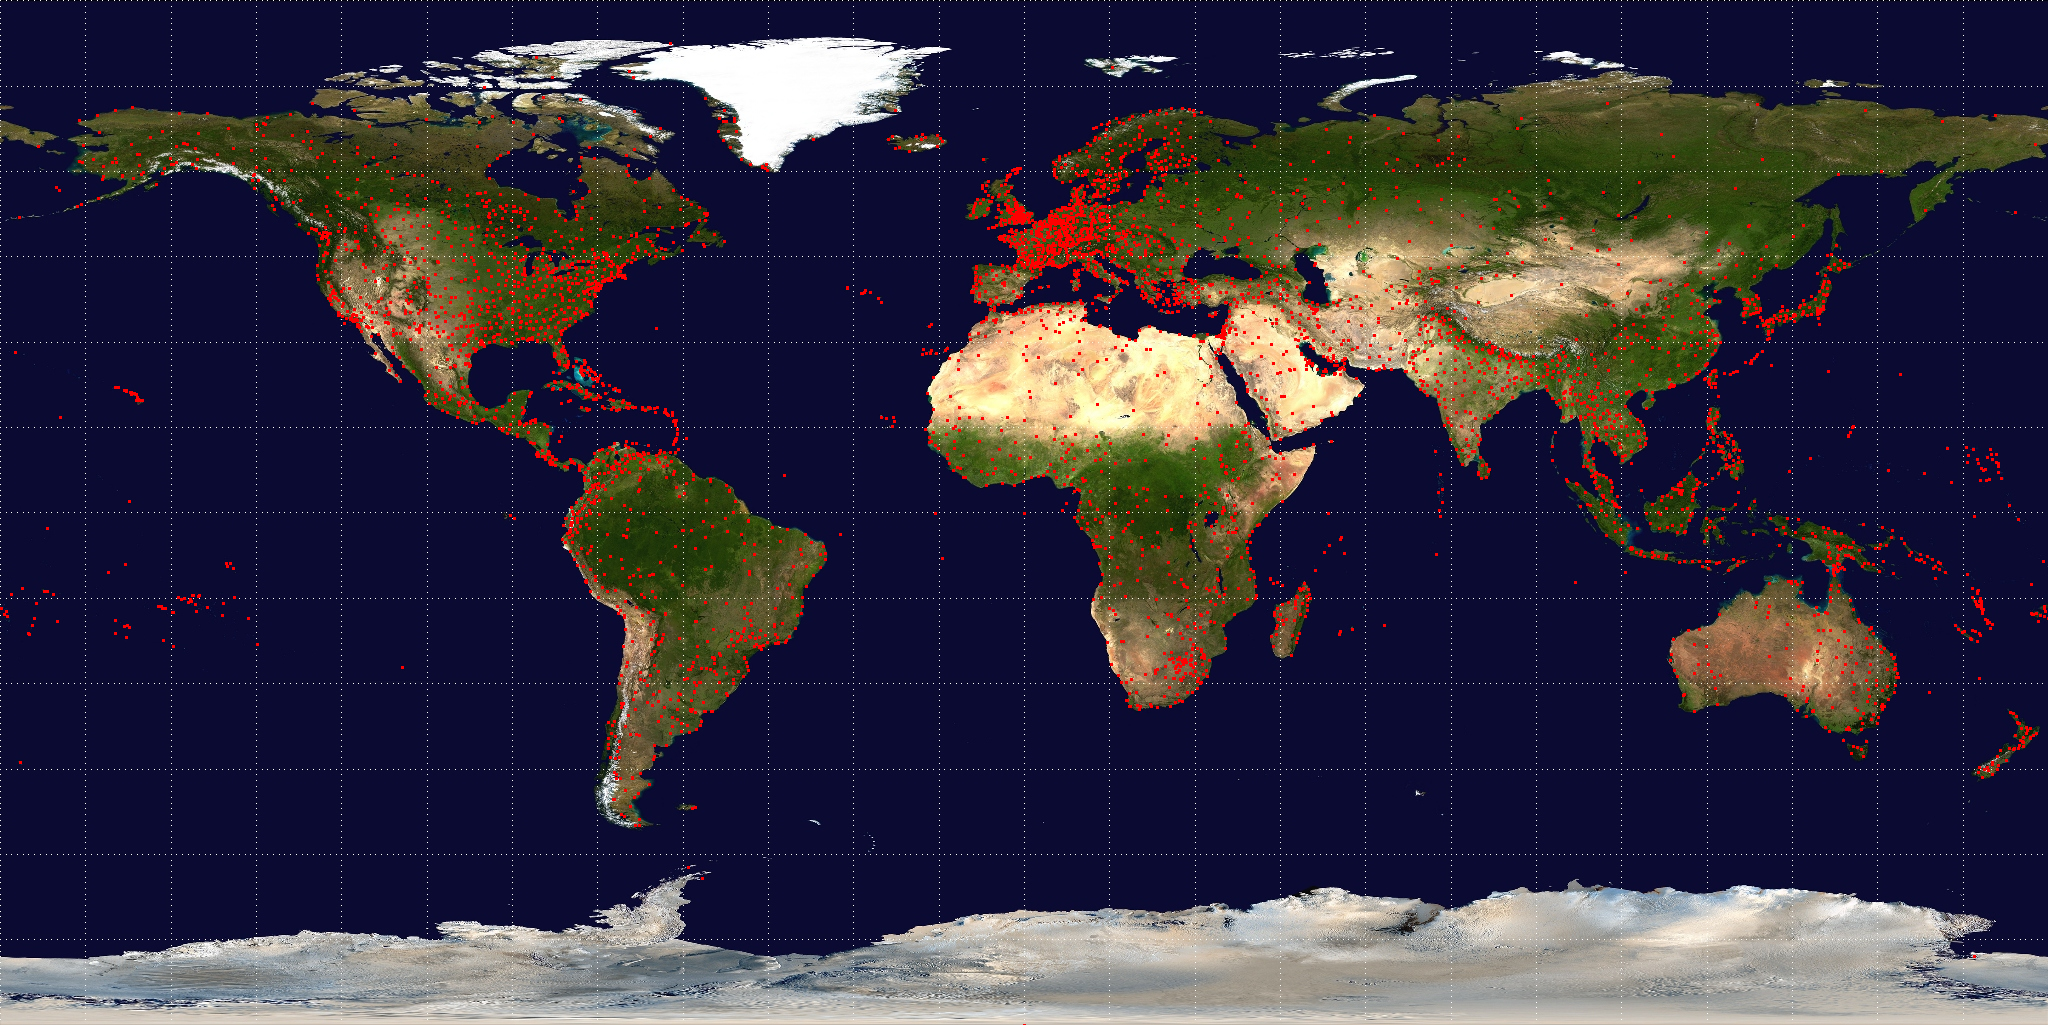
\includegraphics[width=150mm,keepaspectratio=true]{./figures/airports-2048.png}
      \caption{Az OpenFights adatbázisában szereplő repülőterek.}
      \label{fig:figure_repterek}
    \end{figure}

    A rendszer tárolja a repülőterek \textit{nevét}; a \textit{várost}, ahol található; a \textit{szélességi}- és \textit{hosszúsági fokokat}, illetve a \textit{tengerszint feletti magasságot}. Emellett elérhető a repülési hatóságok által használt 3 karakter hosszú \textit{IATA\footnote{International Air Transport Association: Nemzetközi Légi Szállítási Szövetség}/FAA\footnote{Federal Aviation Administration: Szövetségi Légügyi Hivatal (USA)} azonosító} is és az OpenFlights által használt decimális \textit{azonosító} is. A legutolsó, 2014 januári frissítéskor az OpenFlights adatbázisa 9167 repülőteret tartalmazott világszerte, ezt mutatja \aref{fig:figure_repterek}. ábra.

    \begin{table}[ht]
      \footnotesize
      \centering
      \begin{tabular}{ | l | l |}
      \hline
      Attribútum & Leírás \\ \hline
      Airport ID & Egyedi OpenFlights azonosító.\\
      Name & A repülőtér neve.\\
      City & Az a város, amit a repülőtér ,,kiszolgál''.\\
      Country & Az ország vagy terület neve, ahol repülőtér található.\\
      IATA/FAA & 3 betűs FAA kód az USA-beli repülőtereknek vagy 3 betűs IATA kód, minden más esetben.\\
      ICAO & 4 betűs ICAO\footnote{International Civil Aviation Organization: Nemzetközi Polgári Repülési Szervezet} kód.\\
      Latitude & A repülőtér szélességi foka: decimális szám (fokban mérve), általában 6 szignifikáns jegyig.\\
      & A Déli féltekén negatív, az Északin pozitív.\\
      Longitude & A repülőtér hosszúsági foka: decimális szám (fokban mérve), általában 6 szignifikáns jegyig.\\
      & A Nyugati féltekén negatív, a Keletin pozitív.\\
      Altitude & A tengerszint feletti magasság, lábban mérve (1 láb $\sim$ 0,30 méter).\\
      \hline
      \end{tabular}
      \caption{Az OpenFlights adatbázisában elérhető repülőtéri adatok.}
      \label{tab:table_repterek}
    \end{table}

    %----------------------------------------------------------------------------
    \subsection{Repülési útvonalak}
    %----------------------------------------------------------------------------
    \begin{figure}[!ht]
      \centering
      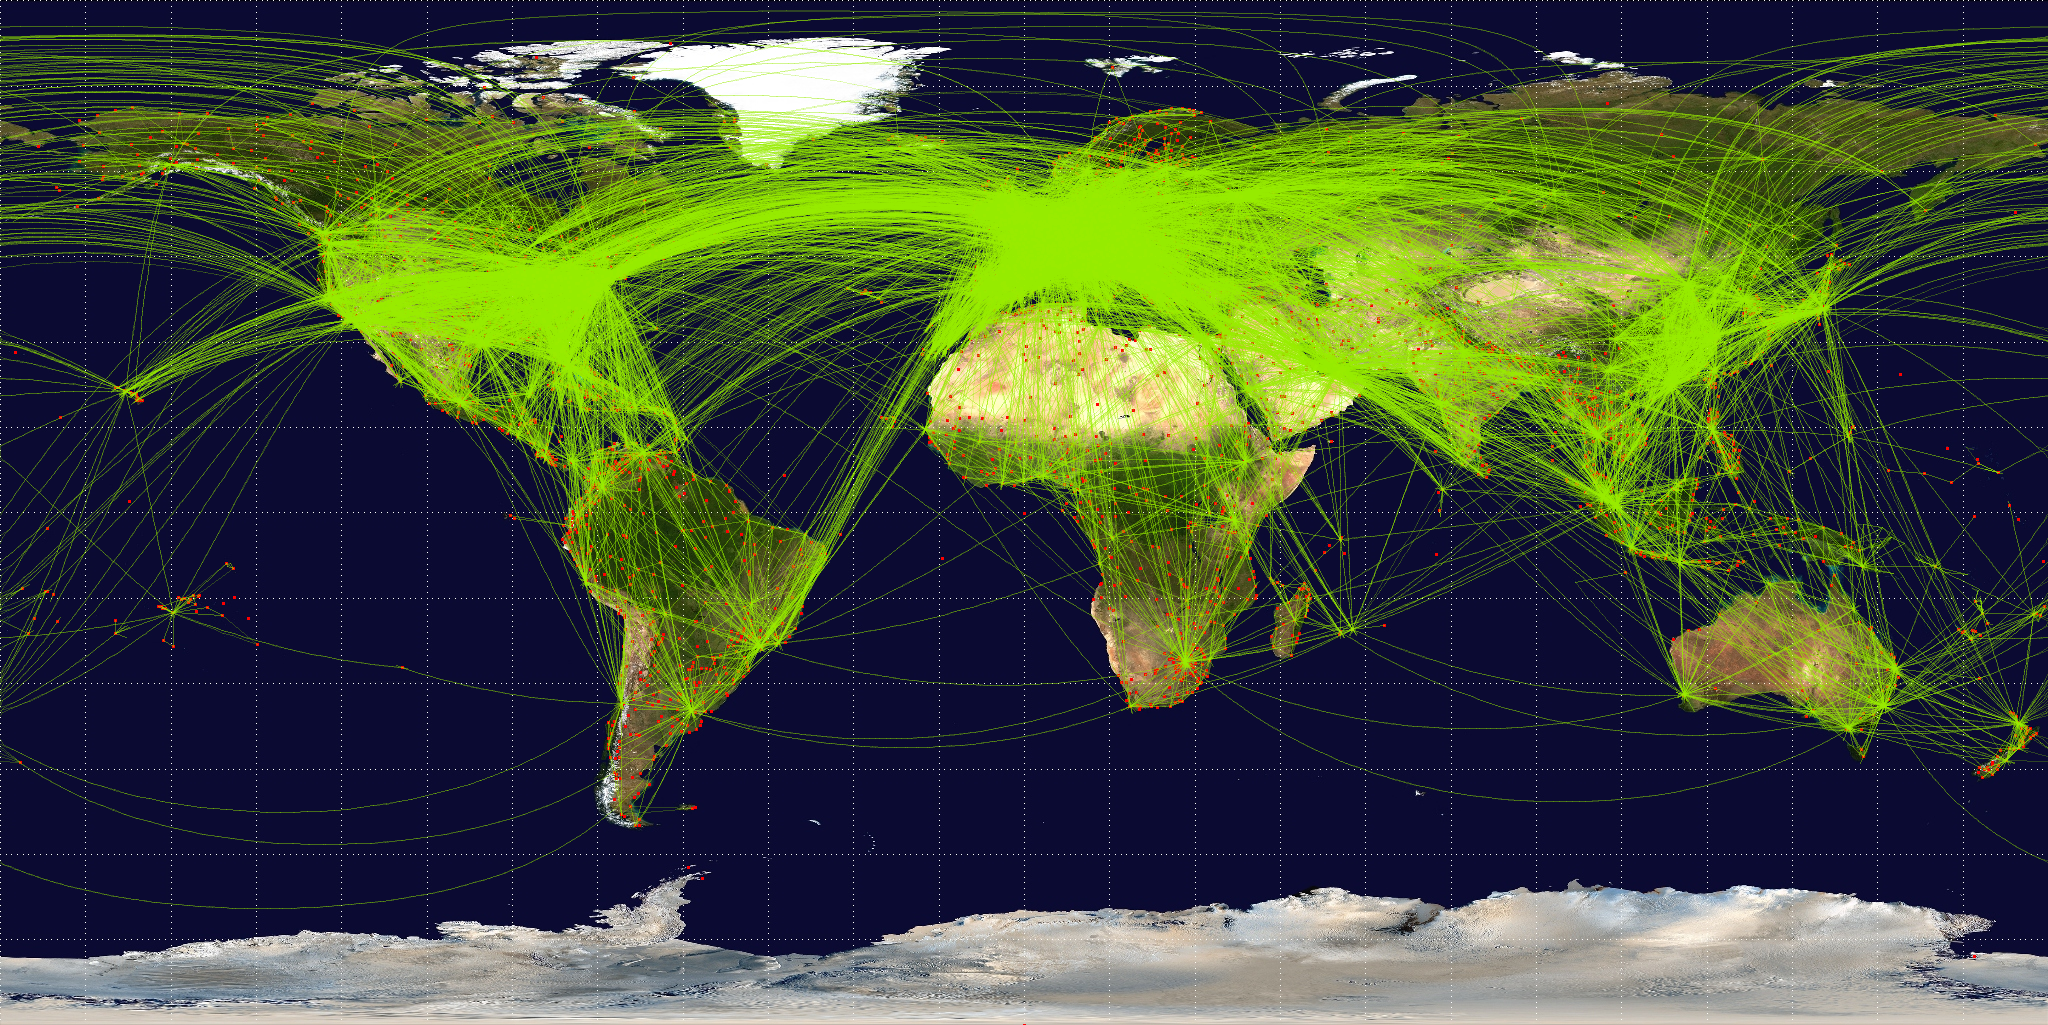
\includegraphics[width=150mm,keepaspectratio=true]{./figures/routes-2048.png}
      \caption{Az OpenFights adatbázisában szereplő repülési útvonalak.}
      \label{fig:figure_repulesiutvonalak}
    \end{figure}

    A repülési útvonalak leírása öt attribútumot tartalmaz: az \textit{üzemeltető repülőtársaság} (név és OpenFlights azonosító); a \textit{forrás repülőtér}; a \textit{cél repülőtér}. Emellett feljegyzik a \textit{megállások számát}\footnote{Az összesen 59637 bejegyzésből 6 esetében van 1 megállás és 1 esetben 2 megállás, ezért ezt az adatot a szimuláció során semmilyen módon nem használom fel.}, illetve az ebben a viszonylatban használt \textit{repülőgép típusokat}. Ha két repülőtér között oda-vissza is van járat, akkor ez az adathalmazban két bejegyzésként jelenik meg. Jelenleg az OpenFlights adatbázisa 59637 útvonalat tartalmazott 3285 repülőtér és 531 társaság\footnote{Ugyan a légitársaság és repülőtér adatbázisokban ennél jelentősen több bejegyzés van, ám azok között vannak nem aktív társaságok, illetve bezárt repülőterek.} között világszerte, ahogy \aref{fig:figure_repulesiutvonalak}. ábra is mutatja.

    \begin{table}[ht]
      \footnotesize
      \centering
      \begin{tabular}{ | l | l |}
      \hline
      Attribútum & Leírás \\ \hline
      Airline & Az üzemeltető társaság 2 betűs (IATA) vagy 3 betűs (ICAO) kódja.\\
      Airline ID & Az üzemeltető társaság egyedi OpenFlights azonosítója.\\
      Source airport & A forrás repülőtér 3 betűs (IATA) vagy 4 betűs (ICAO) kódja.\\
      Source airport ID & A forrás repülőtér egyedi OpenFlights azonosítója.\\
      Destination airport & A cél repülőtér 3 betűs (IATA) vagy 4 betűs (ICAO) kódja.\\
      Destination airport ID & A cél repülőtér egyedi OpenFlights azonosítója.\\
      Codeshare & Igaz, ha a járat ,,codeshare'', azaz nem utasszállító járat, különben üres.\\
      Stops & A megállások szám (nem az átszállásokat jelenti, a ,,0'' jelenti a direkt járatot).\\
      Equipment & A viszonylatban használt repülőgép típusok 3 betűs kódjai.\\
      \hline
      \end{tabular}
      \caption{Az OpenFlights adatbázisában elérhető adatok a repülési útvonalakról.}
      \label{tab:table_repulesiutvonalak}
    \end{table}

    %----------------------------------------------------------------------------
    \subsection{Repülőtársaságok}
    %----------------------------------------------------------------------------
    A repülőtársaságokról tárolt adatok többek között tartalmazzák a hivatalos \textit{IATA azonosítót}; a cég \textit{nevét}; az \textit{országot}, ahol be van jegyezve; illetve, hogy \textit{aktív-e} még a társaság. Emellett természetesen itt is definiáltak egy saját (OpenFlights) \textit{azonosítót}.

    \begin{table}[ht]
      \footnotesize
      \centering
      \begin{tabular}{ | l | l |}
      \hline
      Attribútum & Leírás \\ \hline
      Airport ID & Egyedi OpenFlights azonosító.\\
      Name & A társaság neve.\\
      Alias & A társaság egyéb megnevezése.\\
      IATA & 2 betűs IATA kód.\\
      ICAO & 3 betűs ICAO kód.\\
      Callsign & A társaság hívójele.\\
      Country & Az ország vagy terület neve, ahol a társaság be van jegyezve.\\
      Active & Igaz, ha a társaság jelenleg is, vagy nemrég még működött (nem megbízható).\\
      \hline
      \end{tabular}
      \caption{Az OpenFlights adatbázisában elérhető adatok a repülőtársaságokról.}
      \label{tab:table_repulesitarsasagok}
    \end{table}

  %----------------------------------------------------------------------------
  \section{A szimuláció}
  %----------------------------------------------------------------------------
  \Aref{framework}. fejezetben ismertetett keretrendszert használva vizsgálom meg a fent bemutatott adathalmazon a $\mathcal{S}$ (Shortest algebra), a $\mathcal{L}$ (LeastHop algebra: $\mathcal{L}$ = ($\mathbb{N},~\infty,~+,~\leq$), legkevesebb csomópontot érintő út), az $\mathcal{O}$ (Összekötő-keresés: \ref{osszekoto_kereses}. rész) és a $\mathcal{K}$ (Korai-elfogadó-keresés: \ref{korai_elfogado_kereses}. rész) algebrákat. Mivel az utolsó kettő algebra nem jól viselkedő\footnote{Világos, hogy $\geq$ operátorú algebrák maximumot keresnek, ami ezeknél a konkrét algebráknál maximális utak keresését jelenti. Viszont \aref{max_route}. tétel értelmében csak akkor tudunk maximális utakat keresni, ha a gráf DAG, ami nyilvánvalóan ebben az esetben nem áll fenn, hiszen ez azt jelentené, hogy egy repülőtérről indul soha nem juthatunk vissza ugyanoda.} (lásd \aref{jol_viselkedo}. részt.), ezért csak a $\mathcal{S}$, $\mathcal{L}$, $\mathcal{OS}$, $\mathcal{KS}$, $\mathcal{OL}$ és a $\mathcal{KL}$ algebrákat fogom ténylegesen szimulálni, mert a lexikografikus szorzatban már csak egy adott útvonalhalmazból kell kiválasztani a szorzat első tényezője szerinti legjobbat.

    %----------------------------------------------------------------------------
    \subsection{Az adatok előfeldolgozása}
    %----------------------------------------------------------------------------
    A modellezendő hálózat első megközelítésben a minden csomópontból alkotott $K_{9167}$ teljes gráf. Ez természetesen feleslegesen nagy hálózatot jelent ($9167 \choose 2$ = 42 012 361 élű gráf.), emellett az olyan, leíró jellegű jellemzők, mint a valódi hálózat átmérője, vagy az élösszefüggőség elvesznének. Lévén a repülési hálózat skálafüggetlen -- sok olyan csomópont van, ahova csak adott, kis számú, közeli csomópontokból indulnak járatok, így nem érdemes összekötni távoli csomópontokkal. Ezenkívül a repülésnél vannak olyan szempontok, amelyeket az útvonalválasztásnál figyelembe vesznek, ám én ezek pontos információk hiányában nem tudom kezelni -- pl. csak adott hosszúságú utat tehet meg egy adott típusú repülőgép az üzemanyagtartálya méretétől függően.\\

    A fentiek miatt a szimulált hálózatot a következőképpen határozom meg: pontjai a repülőterek, élei pedig, az adatbázisban szereplő összes, megállás nélküli repülőút. Így magától értetődően csak olyan élek lesznek a szimulációban, amelyek ,,átrepülhetők'', hiszen már átrepülték. Emellett pedig ez a hálózat hűen tükrözi a valóságot, hiszen feltehetjük, hogy csak azon élek nincsenek behúzva, amelyeket repüléstechnikai okokból nem is lehet, különben valaki, valamikor már repült volna azon az úton.

      %----------------------------------------------------------------------------
      \subsubsection{Az élsúlyok meghatározása}
      %----------------------------------------------------------------------------
      Ahogy \aref{prep}. részben kifejtettem, a vizsgálni kívánt algebráktól függően határozom meg az élsúlyozást, valamint a súlyozás során az eredményt nem jelentősen befolyásoló és a futást gyorsító egyszerűsítésekkel élhetek.\\

      A $\mathcal{S}$ algebra miatt szükség van a csomópontok valós távolságára. Ezt a repülőterek szélességi és hosszúsági koordinátái alapján a Haversine formulával számolom. Annak érdekében, hogy pontos, de mégsem túl nagy számokat kapjak a távolságot [km]-ben mért egész számmal jelölöm (az akár [m]-ben mért egytizedes pontosság helyett).\\
      A $\mathcal{L}$ algebra pusztán az élek létét használja fel, így minden él súlya 1.\\
      Az $\mathcal{O}$ algebra a népszerű repülőtereket részesíti előnyben, ami azt jelenti, hogy itt egy csúcs érték $\rightarrow$ élsúly konverzióra van szükség. Minden élet a kezdő- és célcsomópontjának a népszerűsége szerint súlyozunk.\\
      A $\mathcal{K}$ algebra esetén azon az úton fogunk haladni, amin a legtöbben haladtak, így minden élnek a súlyát úgy határozzuk meg, hogy a megfigyelések szerint hányszor repültek az adott viszonylaton.

    %----------------------------------------------------------------------------
    \subsection{A szimuláció menete}
    %----------------------------------------------------------------------------
    A repülési adatok ismeretében nem pontosan \aref{section_simulator}. részben ismertetett módon szimulálok. A gráf élhalmaza a repülési adatokból kapott utak, és ezen a gráfon a 10 legjelentősebb légitársaság útvonalait vizsgálom meg. Bár az előző fejezetben ismertetett szimulátor minden pontpárra előírná az útvonal meghatározását, de jelen esetben a skálafüggetlenség miatt a szimulált utak túlnyomó többsége -- a fokszámeloszlás szerinti ,,farkok'' csúcsai kis fokszámúak -- nem is lehet más, mint a megfigyelt út. Ez eltorzítaná a szimulációt, hiszen azt pozitívan értékeljük, ha pontos a becslés. Ezzel szemben, ha csak a 10 legtöbb járatot üzemeltető társaságot veszem figyelembe, akkor \aref{elossze}. részben leírt \textit{mag}-hoz hasonlóan a lényeget kiemelve tudom vizsgálni a problémát: a 10 legtöbb járatot indító társaság bonyolítja le a repülőutak 24\%-át.

  %----------------------------------------------------------------------------
  \section{Az eredmények}
  %----------------------------------------------------------------------------
  A szimulációs eredmények kiértékelését közönséges táblázatkezelő szoftver segítségével végeztem. Minden algebra által generált gráfról kétféle adathalmazt dolgoztam fel: egy ,,útlistás'' és egy csúcshalmazos reprezentációt.\\

  Az útlistás megadást a generált utak alapján állítottam elő, négy adatot tartalmaz: a \textit{forrás}- és \textit{cél} csomópontokat, valamint a lépésszámot és az algebra szerinti távolságot -- jelen esetben a repülőterek fizikai távolságát. Ezekből az adatokból közvetlenül számíthatók az $AL$ és a $HC$, valamint a $AL-HC$ mutatók.\\

  A csúcshalmazos reprezentáció minden felhasznált csúcsra tartalmazza a csomópont ki- és befokát, valamint ezen mutatók átlagát. Azért volt célszerű előállítani ezt az adathalmazt is, mert innen egyszerűen meghatározható a kétdimenziós fokszámeloszlás, illetve az egydimenziós átlagfokszám-eloszlás. Ebből a forrásból egyszerűen számíthatók a $GD$, a $C$ és az $EC$ mutatók, amiből pedig a $GV$.

    %----------------------------------------------------------------------------
    \subsection{A Shortest algebra}
    %----------------------------------------------------------------------------
    A legrövidebb utakat előnyben részesítő policy algebrája áll várhatóan a legközelebb a valós hálózathoz, hiszen várhatóan a fizikai távolság az útvonalválasztást leginkább befolyásoló tényező.\\

    A $\mathcal{S}$ algebra által generált gráfban 152 pontpár között sikerült javítani a távolságon. Az $AL$ = 152 és $HC$ = 182 így \aref{AL-HC}. képlet szerint $$\text{AL-HC} = 48 \frac{1}{6}.$$\\

    A globális mutatók közül a kétdimenziós fokszámeloszlás \aref{fig:S}. ábrán látható. \Aref{fig:S}. (a) diagramon tízesével csoportosítottam a fokszámokat, azaz az origóhoz legközelebbi jelölés a 10, vagy annál kevesebb fokszámú csúcsokat jelenti. \Aref{fig:S}. (b) ábrán egy ,,kinagyított'' kép látható, csoportosítás nélkül.
    \Histo{shortest}{A $\mathcal{S}$ algebra által generált gráf fokszámeloszlása.}{fig:S}\\

    Látható, hogy a csomópontok ki- és befoka minden pontra közel megegyezik. Ez természetesen várható is volt, hiszen ha két repülőtér között lehetséges a repülés és az egyik irányban létezik is járat, akkor nagy valószínűséggel a másik irányban is repülnek. Az átlagfokszám-eloszlás \aref{fig:S-avg}. ábrán látható. Hasonlóan a másik diagramhoz, itt is egy csoportosított ((a) diagram) és egy kinagyított ((b) diagram) látható. Az ábráról leolvasható, hogy a generált gráf skálafüggetlen, így $DD$ = 1.
    \AvgPlot{shortest}{A $\mathcal{S}$ algebra által generált gráf csomópontonkénti átlagfokszám-eloszlása.}{fig:S-avg}

    A $GD$ (átmérő) mutató 3, mert a legmagasabb lépésszámú út 3 lépést tartalmaz. Az élösszefüggőségi mutatót a felső 20\%-ból számítva $C$ = 16. Az $EC$ (élszám) pontértéke $ln(14578) \approx 9,5872$. Így a Shortest algebrára a $$GV = \frac{DD \cdot GD \cdot C}{ln(EC)} = \frac{1 \cdot 3 \cdot 16}{9,5872} \approx 5,006.$$.

    %----------------------------------------------------------------------------
    \subsection{A LeastHop algebra}
    %----------------------------------------------------------------------------
    Abban az esetben, ha a lépésszám szerint optimalizálunk, a fizikai távolságokon nem tudunk javítani, hiszen a megfigyelt utak közvetlen járatok, azaz egy lépésben elérik a céljukat, ennél pedig nem tudunk jobbat találni. Így $AL=HC$ = 0. Ez természetesen várható volt, nem is a fizikai távolságon javítás a célja a $\mathcal{L}$ algebrának. \Aref{fig:L}. ábrán látszódik a kétdimenziós fokszámeloszlás. Ennél az algebránál a csomópontok több, mint 73\%-a legfeljebb 10 fokú. Nyilván $DD$ = 1.
    \Histo{least}{A $\mathcal{L}$ algebra által generált gráf fokszámeloszlása.}{fig:L}

    Az erősebb skálafüggetlenségből következik, hogy a hálózat ,,magja'' tömörebb, jobban össze vannak fűződve a csomópontok, hiszen ahol csak lehet, közvetlen utat jelöl ki az algebra.
    \AvgPlot{least}{A $\mathcal{L}$ algebra által generált gráf csomópontonkénti átlagfokszám-eloszlása.}{fig:L-avg}

    A $\mathcal{L}$ algebra által generált gráf globális adatai: $GD$ = 1, hiszen minden út 1 lépésből áll. A $C$ = 16. $EC=ln(14396) \approx 9,574$ és így $$GV \approx 1,671.$$.

    %----------------------------------------------------------------------------
    \subsection{A ShortestLeastHop és a LeastHopShortest algebrák}
    %----------------------------------------------------------------------------
    Bár szimuláltam a ShortestLeastHop- és a LeastHopShortest algebrákat is, ám ezek eredménye rendre megegyeznek a LeastHop és a Shortest algebrák eredményeivel, ezért itt nem tüntetem fel. Ez azért lehetséges, mert pl. a Shortest algebra szimulációjával nem feltétlenül egyértelmű a generált gráf. Ha van több legrövidebb út is, akkor véletlenszerűen választunk a legrövidebb utak közül, hiszen a fontos szempont az út hossza, a lépésszám nem számít ebben az esetben. Azt az eljárást, hogy legrövidebb utak közül választunk egyet véletlenszerűen, le lehet egyszerűsíteni úgy, hogy az összes út közül az ,,elsőt'' választjuk (ezt szoftveresen úgyis valamilyen listában vagy tömbben tároljuk), ezzel megspórolhatjuk a véletlenszám-generálást. Így viszont előfordulhat, hogy a tárolt legrövidebb utak közül az ,,első'' éppen a másik algebra szerinti legjobb.

    %----------------------------------------------------------------------------
    \subsection{Az Összekötő-keresés- és Korai-elfogadó-keresés-LeastHop algebrák}
    %----------------------------------------------------------------------------
    Ezek az algebrák teljesen megegyeznek a LeastHop algebrával, ugyanis egy csomópontpár között 1 lépésben csak a közvetlen él van, amit a LeastHop algebra megtalál, így soha nem lesz szerepe az útvonalválasztásban sem az $\mathcal{O}$, sem a $\mathcal{K}$ algebráknak.

  %----------------------------------------------------------------------------
    \subsection{Az Összekötő-keresés-Shortest algebra}
    %----------------------------------------------------------------------------
    Az Összekötő-keresés-Shortest algebra egy pontpár közötti legrövidebb utak közül a legforgalmasabb repülőterek felé haladó utat fogja választani. Ezzel két alapvető tulajdonságot határoz meg, azaz a gráf ,,magja'' és az élszám nagy lesz, hiszen két alternatív út közül azt választja, amelyik a több repülőteret érinti.\\
    \Histo{OS}{Az $\mathcal{OS}$ algebra által generált gráf fokszámeloszlása.}{fig:OS}

    \Aref{fig:OS}. és \aref{fig:OS-avg}. diagramokról leolvasható, hogy a generált gráf skálafüggetlen: $DD$ = 1.
    \AvgPlot{OS}{Az $\mathcal{OS}$ algebra által generált gráf csomópontonkénti átlagfokszám-eloszlása.}{fig:OS-avg}

    Az $AL$ = 152 és $HC$ = 185, így ezek a mutatók szinte megegyeznek a Shortest algebráéval, így $$\text{AL-HC}=47\frac{11}{12}.$$ A $GV$ globális mutató viszont romlott a $\mathcal{S}$ algebráéhoz képest: $$GV \approx 5,01.$$

    A $C$ = 16 és az $EC = ln(14396) \approx 9,57$ értékek megegyeznek, viszont a $GD$ = 3. Az eloszlás szinte teljesen megegyezik a Shortest algebráéval, hiszen ,,azon alapszik'', viszont ez az algebra az összefüggőséget növeli, hiszen minél több csomópontot szeretne érinteni egy adott hosszú úton, így nő a gráf átmérője is. A skálafüggetlenség miatt a ,,mag'' annyira tömör, hogy nem látható az algebra összefüggőségnövelő hatása ($C$ = 16 nem változott).

    %----------------------------------------------------------------------------
    \subsection{A Korai-elfogadó-keresés-Shortest algebra}
    %----------------------------------------------------------------------------
    \Histo{KS}{A $\mathcal{KS}$ algebra által generált gráf fokszámeloszlása.}{fig:KS}
    Ez az algebra a legrövidebb utakból azokat használja, amit előtte -- mások -- már sokan használtak. Ezt természetesen összefüggésben van az Összekötő-keresés algebrával ám itt nem számít a repülőtér tényleges népszerűsége.

    \AvgPlot{KS}{A $\mathcal{KS}$ algebra által generált gráf csomópontonkénti átlagfokszám-eloszlása.}{fig:KS-avg}
    \Aref{fig:KS}. ábrán látható a $\mathcal{KS}$ algebra által generált gráf fokszámeloszlása, \aref{fig:KS-avg}. ábrán pedig a gráf átlagfokszám-eloszlása. A diagramokról leolvasható, hogy $DD$ = 1.

    A $\mathcal{KS}$ algebra mutatói természetesen nagyon hasonlítanak a $\mathcal{S}$ algebráéra, hiszen mindkét esetben a Shortest algebra adja az utakat, amiből választani kell egy legjobbat. Az $AL$ = 152 és $HC$ = 185 így \aref{AL-HC}. képlet szerint $$\text{AL-HC} = 47,95.$$
    A gráf átmérője 4, mert van egy 4 lépéses út a gráfban: $GD$ = 4. A $C$ = 4 megegyezik, ám az $EC=ln(14581) \approx 9,587$, ami valamivel több, mint az egyszerű Shortest algebra esetén, így $$GV \approx 6,67.$$
    \newpage

    %----------------------------------------------------------------------------
    \subsection{Az algebrák értékelése}
    %----------------------------------------------------------------------------
    \renewcommand{\arraystretch}{1.2}
    \begin{table}[ht]
      \centering
        \begin{tabular}{| c || c | c || c || c | c | c | c || c |}
        \hline
        \textbf{Algebra} & $AL$ & $HC$ & $AL-HC$ & $DD$ & $GD$ & $C$ & $EG$ & $GV$\\
        \hline
        Referencia & 0 & 0 & 0 & 1 & 1 & 16 & 9,574705669 & 1,671069645\\
        $\mathcal{S}$ & 152 & 182 & 48,1$\dot{6}$ & 1 & 3 & 16 & 9,587268822 & 5,006639627\\
        $\mathcal{L}$ & 0 & 0 & 0 & 1 & 1 & 16 & 9,574705669 & 1,671069645 \\
        $\mathcal{OS}$ & 152 & 185 & 47,91$\dot{6}$ & 1 & 4 & 16 & 9,574705669 & 5,013208934\\
        $\mathcal{KS}$ & 152 & 185 & 47,95 & 1 & 4 & 16 & 9,58747459 & 6,675376231\\
        \hline
        \end{tabular}
      \caption{A szimulációs eredmények}
      \label{tab:eredmenyek}
    \end{table}

    \Aref{tab:eredmenyek}. táblázatban foglaltam össze a szimulációs eredményeket. Ahogy \aref{metrikak}. részben kifejtettem, egy algebra által generált hálózat pontosságát két tényező határozza meg. Az egyik a $GV$, ami globális mutatókból tevődik össze és minél kisebb az abszolútértéke, annál jobban közelíti meg az eredeti problémát. A másik mutató az $AL-HC$, ami a pontpárokhoz kapcsolódó mutatókat kapcsolja össze és minél nagyobb, annál többet lehet javítani az eredeti hálózathoz képest. Természetesen ezen két mutatót egyszerre kell figyelembe venni, pontosabban a legjobb $GV$ értékű algebrák közül a legmagasabb $AL-HC$ értékű algebra a legjobb.\\

    Az eredményekből arra lehet következtetni, hogy bár a lépésszám szerinti legrövidebb utakat választó $\mathcal{L}$ LeastHop algebra közelíti meg a leginkább az eredeti hálózatot, ezzel az algebrával nem tudunk javítani. Ezzel szemben a fizikai távolság szerint optimalizáló $\mathcal{S}$ Shortest algebra szintén elég pontos közelítése az eredeti hálózatnak, de közel 150 úton lehet még javítani. Emellett meg kell jegyezni, hogy az is kiolvasható a táblázatból, hogy az $\mathcal{OS}$ algebra szinte megegyezik a $\mathcal{S}$ algebra eredményével, ugyanakkor bonyolultabb. Mivel mindkettő elég pontos becslés, feltehető, hogy a repülőtársaságok egy $\mathcal{OS}$ algebrához hasonló szabályrendszer szerint választják meg az útvonalaikat. Ebben az esetben érdemes lenne nekik áttérni az egyszerű $\mathcal{S}$ algebrára, hiszen a két hálózat szinte megegyezik, és a $\mathcal{S}$ útvonalválasztása jóval egyszerűbb.

  %----------------------------------------------------------------------------
  \section{Összefoglaló}
  %----------------------------------------------------------------------------
  Ebben a fejezetben \aref{framework}. fejezetben leírt keretrendszert használva megvizsgáltam egy valós hálózatot az \href{http://openflights.org/}{openflights} repülési adatbázisát felhasználva. A szimulációs keretrendszerben meghatározott lépéseket elvégeztem, a szükséges módosításokat megtettem, ahol a probléma miatt erre szükség volt. A repülési adatbázis alapján létrehoztam az irányított, vektor-súlyozott gráfot, az élsúlyokat a vizsgálandó algebrák alapján számítottam ki és rendeltem az élekhez.\\

  A kész tervet a saját magam írt szimulátor szoftverrel hajtottam végre, az eredményeket közönséges táblázatkezelővel elemeztem. Megvizsgáltam a Shortest ($\mathcal{S}$), a LeastHop ($\mathcal{L}$), az Összekötő-keresés ($\mathcal{O}$) és a Korai-elfogadó-keresés ($\mathcal{K}$) algebrákat. Mivel az utóbbi kettő nem jól viselkedő algebra, ezeket csak a Shortest és a LeastHop algebrákkal való lexikografikus szorzatukban vizsgáltam. Az Összekötő-keresés-LeastHop ($\mathcal{OL}$) és a Korai-elfogadó-keresés-LeastHop ($\mathcal{KL}$) algebrákat, valamint a Shortest-LeastHop ($\mathcal{SL}$) és LeastHop-Shortest ($\mathcal{LS}$) algebrákat nem kellett vizsgálnom. Az első kettőnek elméleti megfontolások alapján nincs új információtartalma, utóbbi kettő pedig előáll a külön-külön szimulált algebrák speciális alakjaként.\\

  A korábban definiált pontrendszert felhasználva beazonosítottam a repülési adatok alapján legtöbb javítási lehetőséget nyújtó algebrát, a Shortest algebrát. Ez elég pontosan becsli az eredetei megfigyelt hálózatot, ugyanakkor megmutat olyan lehetőségeket, amik mentén javíthatunk a jelenlegi útvonalválasztáson.
  Emellett rávilágítottam a tényre, hogy az $\mathcal{OS}$ algebrát, amit akár a valóságban is használhatnak -- elég jó becslése az eredeti hálózatnak -- nem érdemes használni, mert a $\mathcal{S}$ algebra egyszerűbb és pontosabb becslés, azaz erre le lehetne cserélni a jelenleg alkalmazott szabályrendszert.
